\section{SiPM Simulation Analysis}

To do the analysis using the SiPM simulation, we simply measure the total output of the SiPM over a light pulse and compare it to the number of input photons. Since there is a degree of randomness we will use the average pulse over several inputs. Compared to using test beam data the analysis with the simulation is simple. In test beam the energy of the particle is spread over several SiPMs while in the simulation we have a very fine control of the input energy to the single SiPM. With a plot of input number of photons vs SiPM output charge we then create a correction curve that is necessary to make the graph linear. This is process for doing a non-linearity analysis using test beam data so we can compare the two correction curves to see if there is agreement. With other analyses it is common to simply divide out the cross talk. Given that there is a $15.4\%$ chance of crosstalk with a large signal of several thousand photons it is assumed that $15.4\%$ of the signal from the SiPM is due to cross talk so that number is simply divided out. This means the majority of the effects that the correction curve is compensating for is saturation. With the simulation we can simply turn off cross talk but it is still useful to compare non-linear curves with cross talk, cross talk turned off, and cross talk divided out.

\begin{figure}
\centering
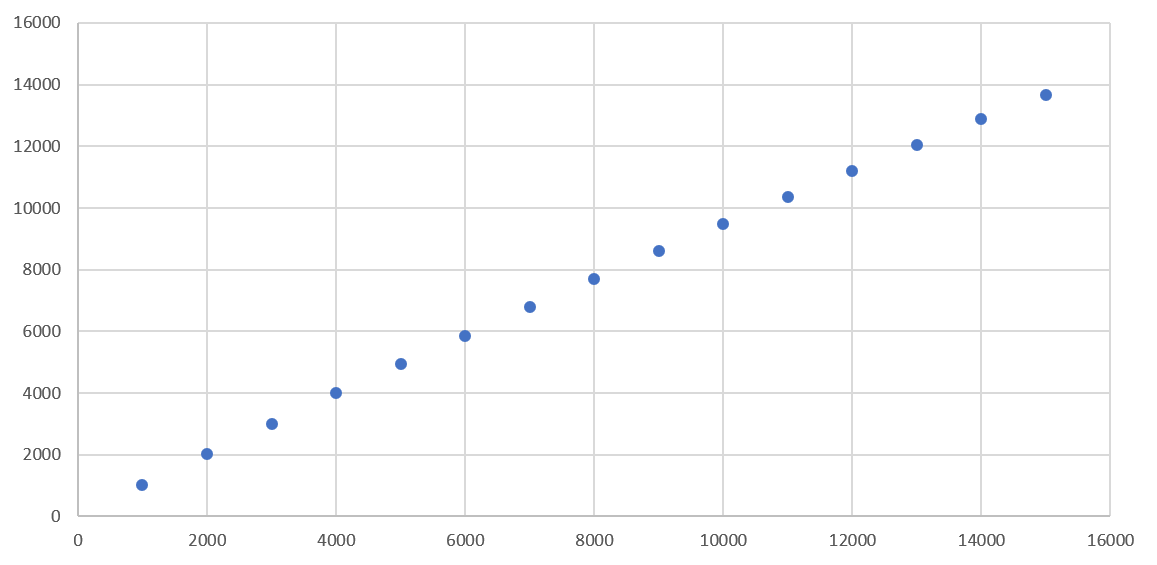
\includegraphics[width=\linewidth]{Figures/SimNon.png}
\caption{Graph of number of incident photons vs output charge of the SiPM simulation. Given the units of the simulation a perfectly linear device would have all data points falling on the y=x line but as shown as the number of incident photons is increased the data points fall short of this line.}
\label{fig:SimNon}
\end{figure}

%I am working on creating these plots with high resolution and statistics. Once they are done I will make a correction curve. Is there accepted data I can compare it too?

%Another analysis I have plots for is the effects of changing the rehcarge time of the pixels. 

Using the simulation we can also look at the pulse shape of the SiPM. One of the main things that is necessary to look at is does the pulse shape change significantly with a change in input energy.

\begin{figure}
\centering
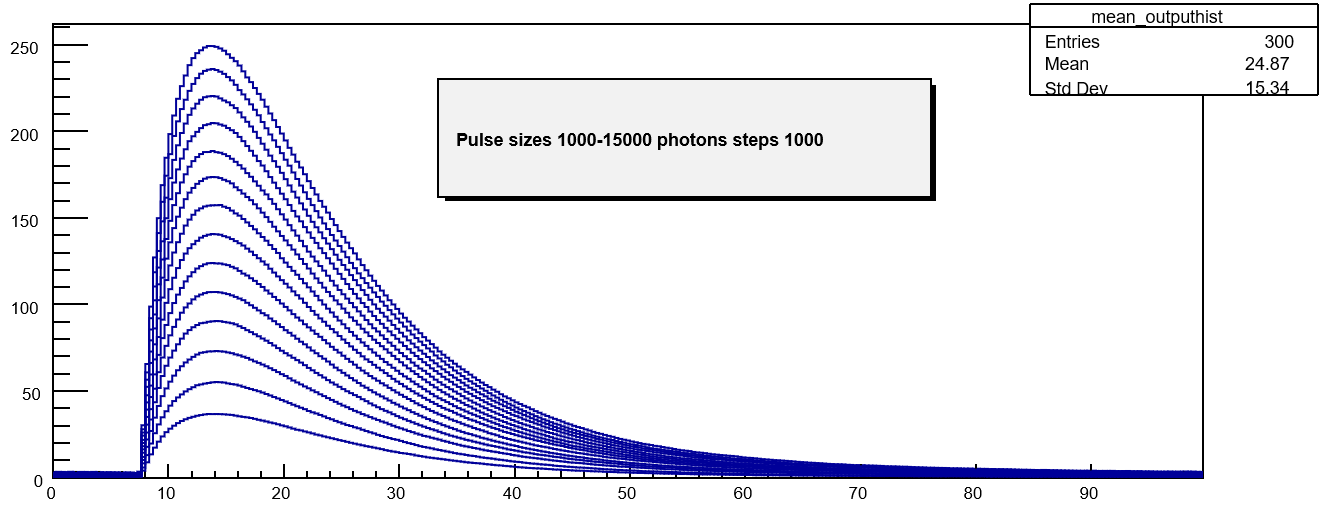
\includegraphics[width=\linewidth]{Figures/SimPul.png}
\caption{Pulse shapes from the SiPM simulation. They are stacked on top of each other to highlight any differences from an increase input photon count.}
\label{fig:SimPul}
\end{figure}

%I have plots for this analysis but I am not quite sure how to show it. I have plots showing normalized output pulses of different input energies and log plots of them but I am not sure of the best way to showcase it. Is there a numerical analysis to show how close they are?